\documentclass[11pt,a4paper]{article}
\usepackage[utf8]{inputenc}
\usepackage{amsmath,amsfonts,amssymb}
\usepackage{graphicx}
\usepackage{geometry}
\geometry{margin=1in}
\usepackage{booktabs}
\usepackage{hyperref}
\usepackage{float}
\usepackage{xcolor}

\title{\textbf{EE3621: Digital Signal Processing} \\ \Large Lecture 25: DSP in Communications — Modulation, Detection \& Matched Filter \\ \large (III B.Tech EEE)}
\author{Lecture Notes (40-Minute Plan)}
\date{}

\definecolor{darkbg}{HTML}{0d121f}
\definecolor{lighttext}{HTML}{e2e8f0}
\definecolor{primary}{HTML}{8b5cf6}
\definecolor{secondary}{HTML}{0dd5c5}

\pagecolor{darkbg}
\color{lighttext}

\hypersetup{
    colorlinks=true,
    linkcolor=secondary,
    urlcolor=secondary
}

\begin{document}

\maketitle

\section{Lecture Plan (40 Minutes Breakdown)}
\begin{itemize}
    \item \textbf{00:00 -- 05:00 (5 mins):} Digital Modulation Review (BPSK, QPSK, QAM).
    \item \textbf{05:00 -- 12:00 (7 mins):} Pulse Shaping \& Inter-Symbol Interference (ISI); Raised Cosine and Square-Root Raised Cosine filters.
    \item \textbf{12:00 -- 22:00 (10 mins):} Matched Filter \& Correlation Receiver; SNR maximization proof.
    \item \textbf{22:00 -- 28:00 (6 mins):} Equalization techniques (Zero-Forcing, MMSE, DFE).
    \item \textbf{28:00 -- 35:00 (7 mins):} OFDM Fundamentals, Cyclic Prefix, FFT/IFFT architecture, and Standards.
    \item \textbf{35:00 -- 40:00 (5 mins):} Checkpoints \& Worked Examples.
\end{itemize}

\noindent\rule{\textwidth}{0.5pt}

\section{Digital Modulation Review}
In modern communication systems, digital information is transmitted by modulating the amplitude and phase of a carrier.

\subsection{Complex Baseband Representation}
Any passband signal can be mathematically represented in terms of its complex baseband equivalent.
Let the passband signal be $x(t)$:
\begin{equation}
x(t) = \text{Re}\{ s(t) e^{j 2\pi f_c t} \}
\end{equation}
In discrete time, a modulated symbol is sampled as $s_i[n]$:
\begin{equation}
s_i[n] = I_i[n] + j Q_i[n]
\end{equation}
where $I_i[n]$ is the In-phase component and $Q_i[n]$ is the Quadrature component.

\subsection{Constellations}
\begin{itemize}
    \item \textbf{BPSK:} Symbols from $\{+A, -A\}$ (1 bit/symbol).
    \item \textbf{QPSK:} Symbols from $\{\pm A \pm jA\}$ (2 bits/symbol).
    \item \textbf{QAM:} Varies amplitude and phase, $\log_2(M)$ bits/symbol.
\end{itemize}

\section{Pulse Shaping and ISI}

\begin{figure}[H]
    \centering
    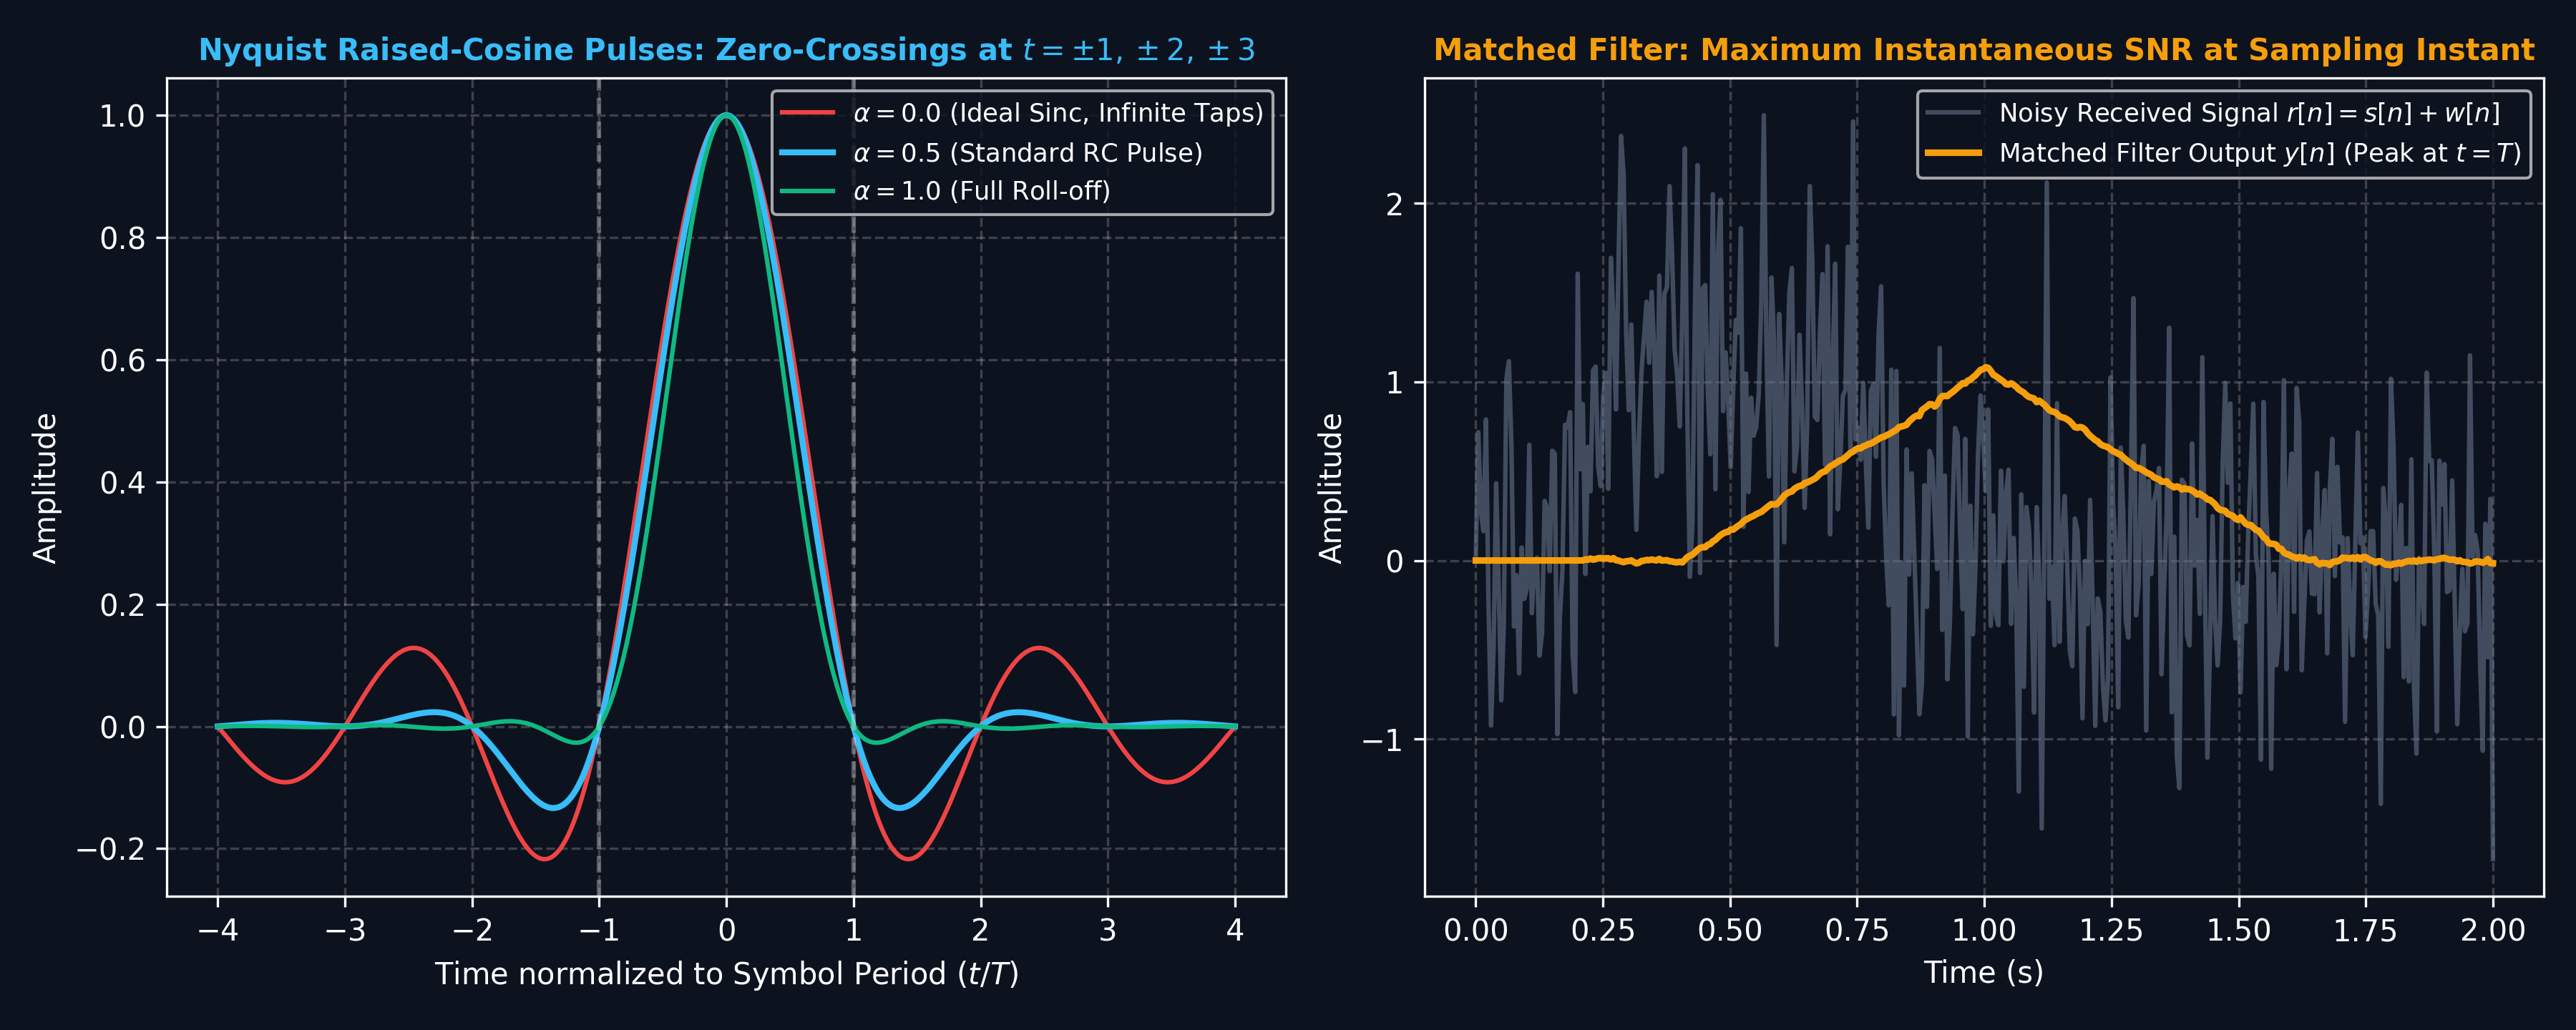
\includegraphics[width=0.85\textwidth]{images/raised_cosine_pulse_and_isi.png}
    \caption{Nyquist Raised-Cosine Zero-ISI Pulses and Matched Filter Output Peak Instantaneous SNR.}
\end{figure}

\begin{figure}[H]
    \centering
    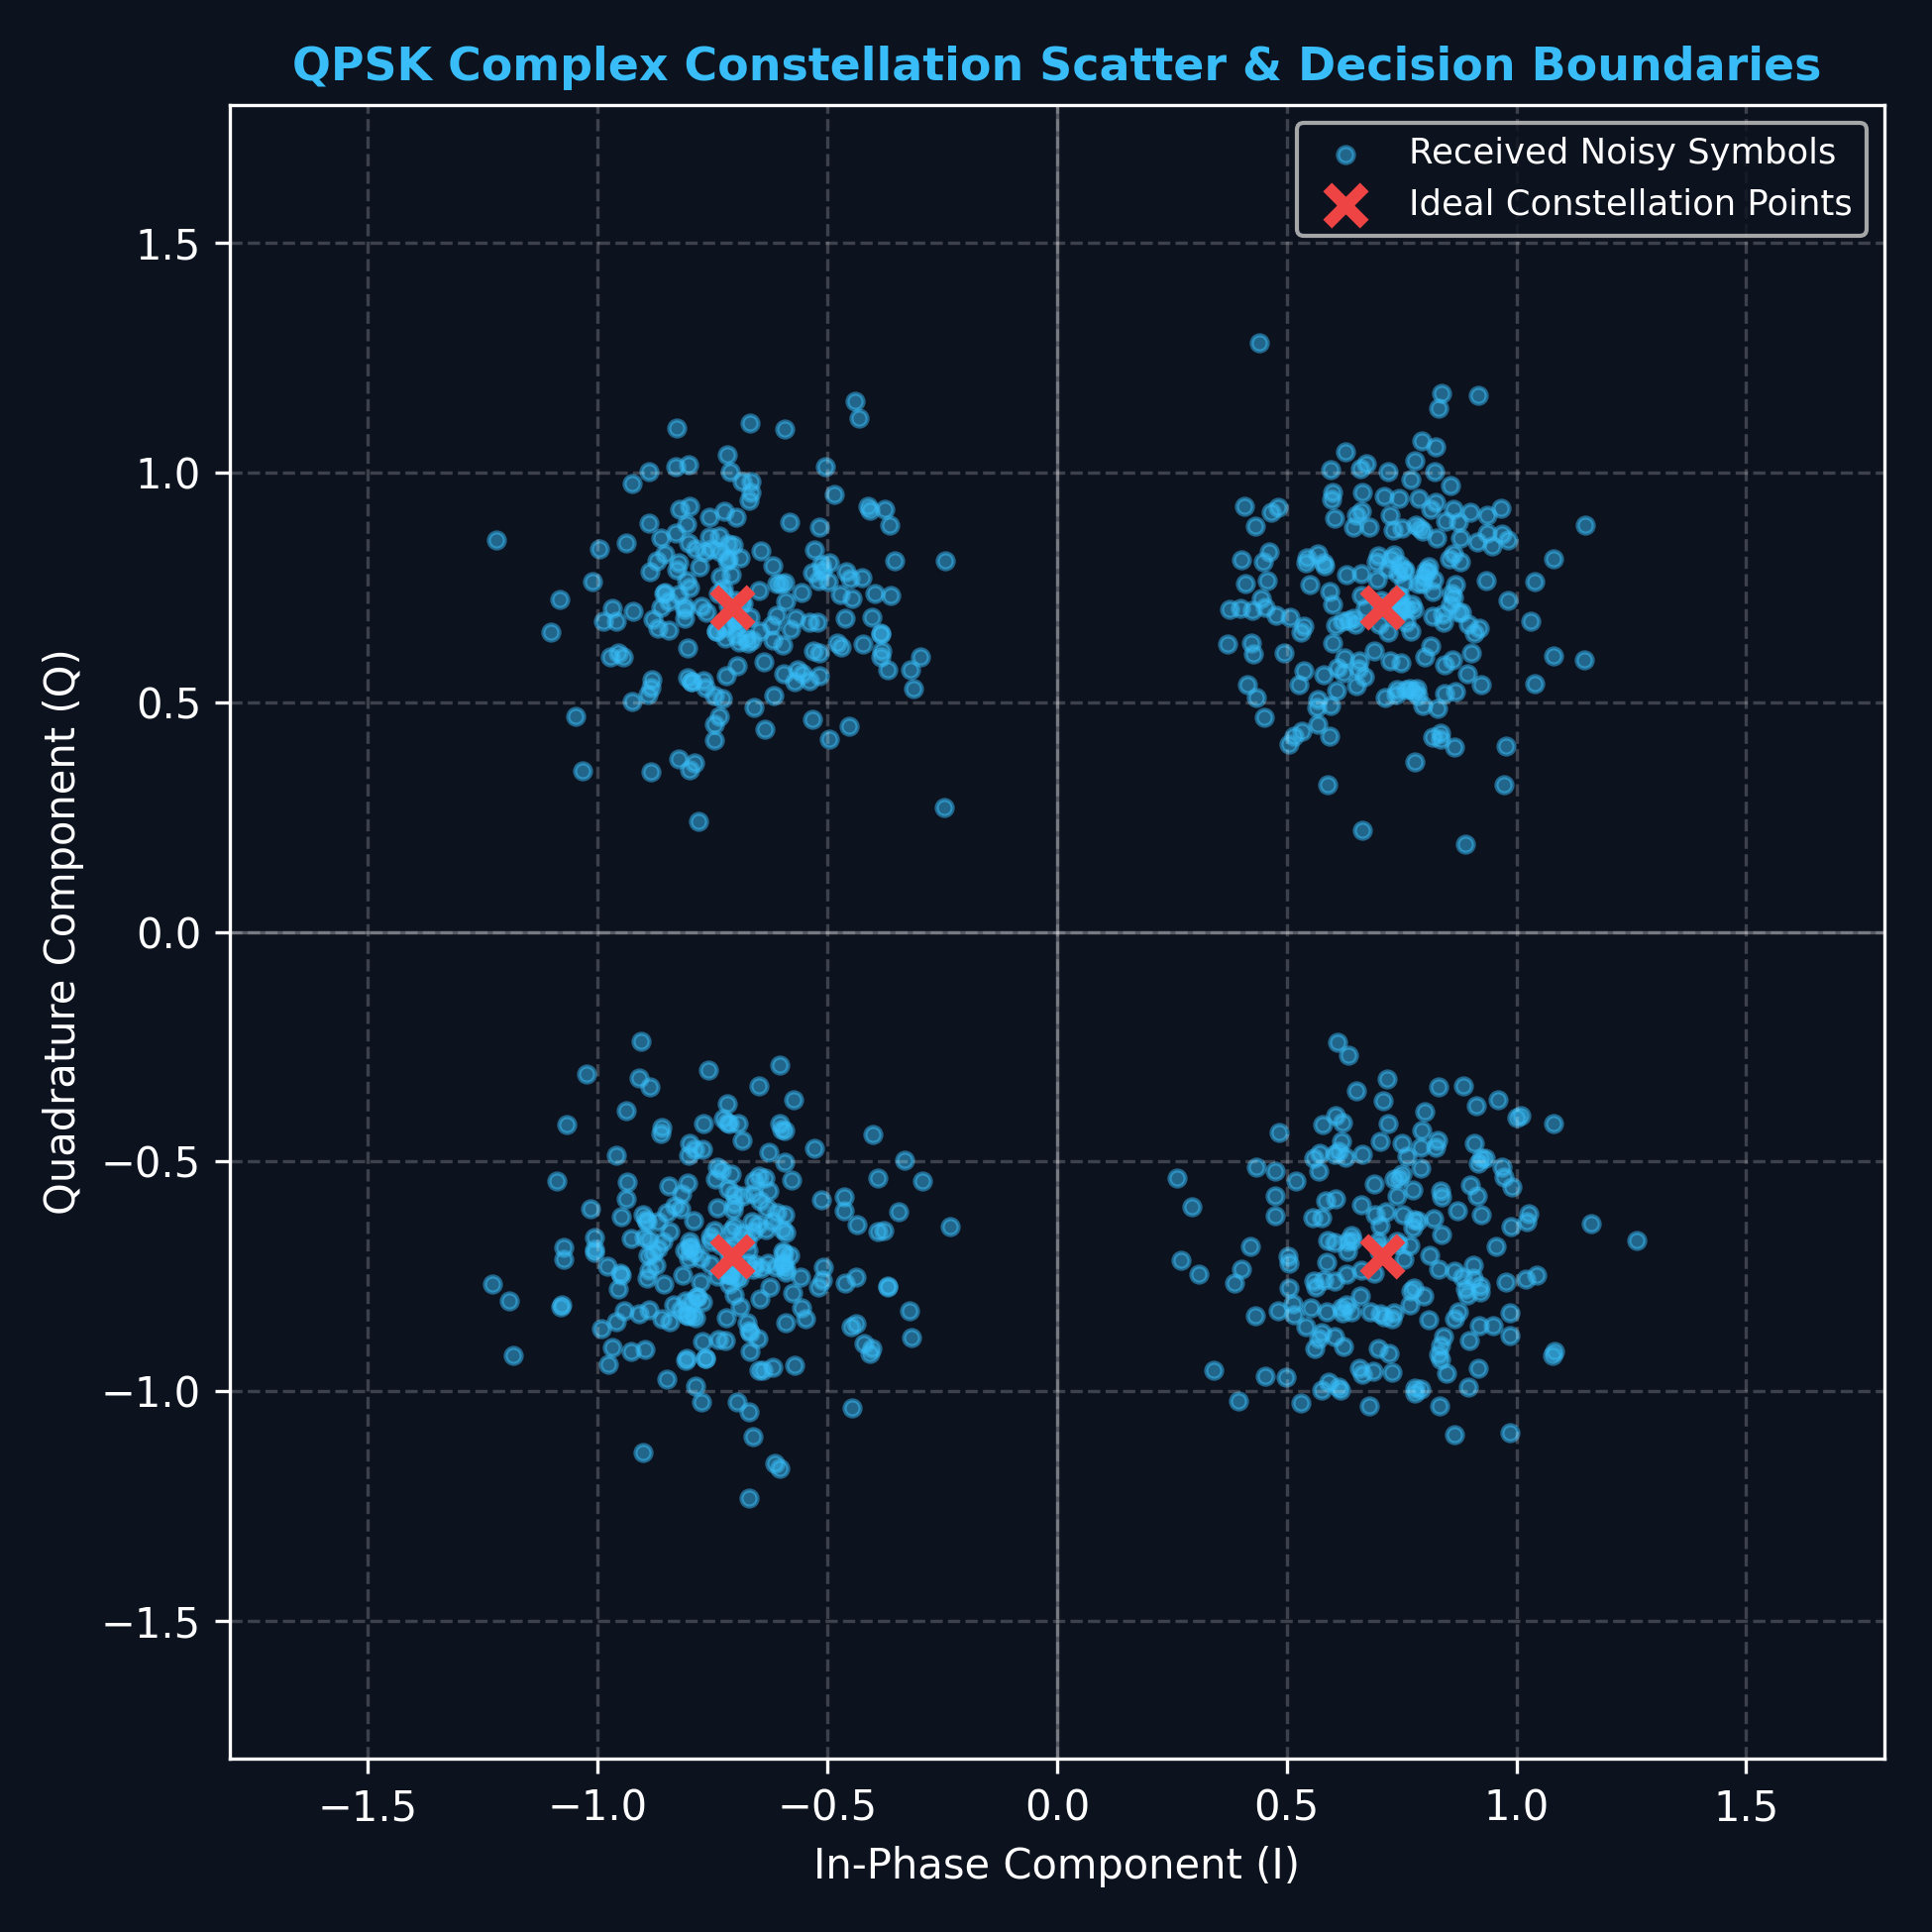
\includegraphics[width=0.65\textwidth]{images/qpsk_constellation_and_eye_diagram.png}
    \caption{QPSK Complex Constellation Scatter Diagram with Noise and Decision Boundaries.}
\end{figure}


\subsection{The ISI Problem}
The received signal is:
\begin{equation}
y(nT) = s[n] p(0) + \sum_{k \neq n} s[k] p((n-k)T)
\end{equation}
The second term is the Inter-Symbol Interference (ISI).

\subsection{Nyquist Criterion for Zero-ISI}
To achieve zero ISI, the time-domain pulse must satisfy:
\begin{equation}
p(nT) = \begin{cases} 1 & n = 0 \\ 0 & n \neq 0 \end{cases}
\end{equation}

\subsection{Raised Cosine Filter}
The absolute bandwidth required is given by:
\begin{equation}
B = \frac{1+\alpha}{2T}
\end{equation}
where $\alpha \in [0,1]$ is the roll-off factor.

\section{The Matched Filter}
The Matched Filter maximizes the Signal-to-Noise Ratio (SNR) at the sampling instant.
\begin{equation}
h(t) = s^*(T_0 - t)
\end{equation}
Discrete form:
\begin{equation}
h[n] = s^*[L-n]
\end{equation}

\subsection{Formal Proof of SNR Maximization}
The SNR at the sampling instant is:
\begin{equation}
\text{SNR} = \frac{\left| \int_{-\infty}^{\infty} H(f) S(f) e^{j 2\pi f T_0} df \right|^2}{\frac{N_0}{2} \int_{-\infty}^{\infty} |H(f)|^2 df}
\end{equation}
Applying the Cauchy-Schwarz inequality:
\begin{equation}
\left| \int H(f) S(f) e^{j 2\pi f T_0} df \right|^2 \leq \left( \int |H(f)|^2 df \right) \left( \int |S(f)|^2 df \right)
\end{equation}
Equality is achieved when $H(f) = k S^*(f) e^{-j 2\pi f T_0}$. The maximum SNR is:
\begin{equation}
\text{SNR}_{\max} = \frac{2 E_s}{N_0}
\end{equation}

\section{Channel Equalization}
\begin{itemize}
    \item \textbf{Zero-Forcing:} $H_{eq}(f) = 1 / H_{channel}(f)$ (Enhances noise).
    \item \textbf{MMSE:} $H_{MMSE}(f) = \frac{H^*(f)}{|H(f)|^2 + N_0/E_s}$.
    \item \textbf{DFE:} Uses past decisions to subtract ISI cleanly.
\end{itemize}

\section{OFDM Fundamentals}
Orthogonal Frequency Division Multiplexing divides the high-rate stream into many parallel low-rate subcarriers.
\begin{itemize}
    \item \textbf{Cyclic Prefix (CP):} Converts linear convolution to circular convolution, eliminating ISI.
    \item \textbf{IFFT/FFT:} Used as efficient modulator and demodulator.
\end{itemize}

\section{Summary of Key Formulas}
\begin{table}[H]
\centering
\begin{tabular}{@{}ll@{}}
\toprule
Concept & Formula \\ \midrule
Complex Baseband & $s_i[n] = I_i[n] + j Q_i[n]$ \\
Raised Cosine Bandwidth & $B = \frac{1+\alpha}{2T}$ \\
Matched Filter & $h[n] = s^*[L-n]$ \\
Matched Filter SNR & $\text{SNR} = 2E_s/N_0$ \\
MMSE Equalizer & $H_{MMSE}(f) = \frac{H^*(f)}{|H(f)|^2 + N_0/E_s}$ \\ \bottomrule
\end{tabular}
\end{table}

\section{Checkpoints}
Detailed step-by-step solutions for Checkpoints are available in the full markdown notes.
\end{document}
